\documentclass{beamer}
%\documentclass[handout]{beamer}
%\documentclass[handout,notes=show]{beamer}

\usetheme{Frankfurt}
\usecolortheme{dolphin}
\beamertemplatenavigationsymbolsempty

\usepackage{amsmath, amssymb, amsfonts, tikz}
\usepackage[utf8]{inputenc}
\usepackage[T1]{fontenc}
\usepackage[english]{babel}
\usepackage{tikz}
\usetikzlibrary{calc}

\DeclareMathOperator{\Gal}{Gal}
\DeclareMathOperator{\cl}{cl}
\DeclareMathOperator{\CC}{\mathbf{C}}
\DeclareMathOperator{\ZZ}{\mathbf{Z}}
\DeclareMathOperator{\QQ}{\mathbf{Q}}
\DeclareMathOperator{\RR}{\mathbf{R}}
\DeclareMathOperator{\p}{\mathfrak{p}}
\DeclareMathOperator{\pp}{\mathfrak{P}}
\DeclareTextFontCommand{\emph}{\bfseries}

\author{Alex J. Best}
\institute{WIMP 2014}
\date{29/11/2014}
\title{Singular Moduli}

\begin{document}

\section{Introduction}

\frame{\titlepage
\note{
so if you dont know me already perhaps i should explain that i was at warwick until this academic year and so I'd
like to start by thanking the organisers for giving me the excuse to come back and see you all,
and also for the chance to tell you about this very interesting topic.
}
}

\begin{frame}
\frametitle{In this talk:}
\note{
Will talk about some special values of a special function, their properties and the surprising consequences.
I will prove very little, instead try and give a flavour of a few topics that I find interesting.
}
\tableofcontents
\end{frame}

\begin{frame}
\note{
}
Observations (Hermite, 1859):
\[
\begin{aligned}
\action<1->{
e^{\pi\sqrt{43}} &\approx 884736743.999777466 \\}
\action<4->{
&\approx 12^3(9^2 - 1)^3 + 744 - 10^{-4}\cdot 2.225\ldots \\}
\action<2->{
e^{\pi\sqrt{67}} &\approx 147197952743.999998662454 \\}
\action<4->{
&\approx 12^3(21^2 - 1)^3 + 744 - 10^{-6}\cdot 1.337\ldots \\}
\action<3->{
e^{\pi\sqrt{163}} &\approx 262537412640768743.99999999999925007\\}
\action<4->{
&\approx 12^3(231^2 - 1)^3 + 744 - 10^{-13}\cdot 7.499\ldots}
\end{aligned}
\]
\end{frame}

\section{Background}

\begin{frame}{Some definitions}
\note{
After Alex's (excellent?) talk will go easy on the background, but if anything remains unclear please do stop me and ask.
}
\begin{block}{Definition}
A finite Galois extension $L|K$ is \emph{abelian} extension if $\Gal(L|K)$ is abelian.\\
\end{block}
\pause
Examples: \\%TODO
\pause
Non-examples: \\%TODO

%TODO ring of integers of a number field, introduced to fix problem of non-unique factorisation
\end{frame}

\begin{frame}{The ideal class group}
\note{definition central to ANT}
Given a number field $K$ we let
\[
I(\mathbf{Z}_K) = \{\}
\]
be the set of \emph{fractional} ideals of $\mathbf{Z}_K$.
\pause
This is an (abelian) group!
\pause
The set
\[
P(\mathbf{Z}_K)= \{a\mathbf{Z}_K : a\in K\}
\]
of \emph{principal} ideals is a subgroup.
\pause
\begin{block}{Definition}
The \emph{ideal class group} of a number field $K$ is the quotient
\[
\cl(\mathbf{Z}_K) = I(\mathbf{Z}_K)/P(\mathbf{Z}_K).
\]
\end{block}
\pause
$\cl(\mathbf{Z}_K)$ \emph{measures} how far $\mathbf{Z}_K$ is from having unique factorisation.
\end{frame}

\section{The Hilbert class field}
\begin{frame}{The Hilbert class field (of an imaginary quadratic field)}
\note{This definition is specific to imaginary quadratic fields, for more general fields we need another condition that turns out to be vacuous here so I left it out to keep things simple.

Explain what maximal means in this context.
}
Let $K$ be an \emph{imaginary quadratic} number field, i.e. $K = \mathbf{Q}(\sqrt{-n})$ for some $n \in \mathbf{Z}_{\ge 1}$.
\pause
\begin{block}{Definition}
An extension $L|K$ is \emph{unramified} if for all prime ideals $\p$ of $\mathbf{Z}_K$ we have a factorisation
\[
\p\mathbf{Z}_L = \pp_1\pp_2\cdots \pp_n
\]
into \emph{distinct} prime ideals $\pp_i$ of $\mathbf{Z}_L$.
\end{block}
\pause
\begin{block}{Definition}
The \emph{Hilbert class field} of $K$ is the maximal unramified abelian extension of $K$.
\end{block}
\end{frame}

\begin{frame}{The Hilbert class field (of an imaginary quadratic field)}
\note{
Why do we care?
}
\begin{block}{Definition}
The \emph{Hilbert class field} of $K$ is the maximal unramified abelian extension of $K$.
\end{block}
\begin{block}{Examples}
\begin{table}
\centering
\begin{tabular}{| l | l | l |}
  \hline
  $K$ & Hilbert class field $L$ & $\Gal(L|K)$ \\
  \hline
  $\mathbf{Q}(\sqrt{-1})$ & $\mathbf{Q}(\sqrt{-1})$ & 1\\
  \pause
  $\mathbf{Q}(\sqrt{-31})$ & $\mathbf{Q}(\sqrt{-31})[x]/(x^3 + x - 1)$ & $C_3$\\
  \pause
  $\mathbf{Q}(\sqrt{-159})$ & $\begin{aligned} \mathbf{Q}&(\sqrt{-159})[x]/(x^{10} - 3x^9 + 6x^8\\
  &- 6x^7 + 3x^6 + 3x^5 - 9x^4 \\
  &+ 13x^3 - 12x^2 + 6x - 1)\end{aligned}$ & $C_{10}$\\
  \pause
  $\mathbf{Q}(\sqrt{-163})$ & $\mathbf{Q}(\sqrt{-163})$ & 1\\
  \hline
\end{tabular}
\end{table}
\end{block}
\end{frame}

\begin{frame}{The Artin reciprocity theorem for the Hilbert class field}
\note{what a mouthful, this explains the name hilbert _class_ field, this theorem as stated is true for all number fields!}
\begin{block}{Theorem}
If $K$ is a number field and $L$ is its Hilbert class field then
\[
\cl(\ZZ_K) \cong \Gal(L|K).
\]
\end{block}
\begin{center}
\begin{tikzpicture}[node distance = 1.7cm, auto]
  \node (Q) {$\mathbf{Q}$};
  \node (K) [above of=Q] {$K$};
  \node (L) [above of=K] {$L$};
  \draw[-] (Q) to node {} (K);
  \draw[-] (K) to node [swap] {$\Gal(L|K)$} (L);
\end{tikzpicture}
\end{center}
\end{frame}

%TODO example ? big extension must be ramified

\begin{frame}{Lattices}
\begin{block}{Definition}
A \emph{lattice} is an additive subgroup of $\CC$ that is isomorphic to $\ZZ^2$.
\end{block}
\begin{figure}
\centering
  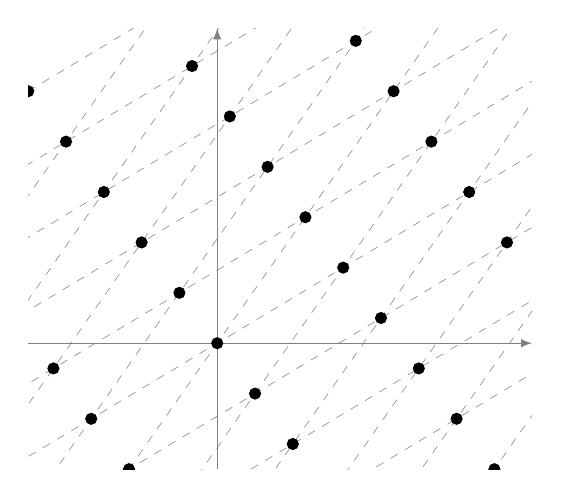
\begin{tikzpicture}[scale=0.8, every node/.style={scale=0.7}]
    \coordinate (Origin)   at (0,0);
    \coordinate (XAxisMin) at (-3,0);
    \coordinate (XAxisMax) at (5,0);
    \coordinate (YAxisMin) at (0,-2);
    \coordinate (YAxisMax) at (0,5);
    \draw [thin, gray,-latex] (XAxisMin) -- (XAxisMax);% Draw x axis
    \draw [thin, gray,-latex] (YAxisMin) -- (YAxisMax);% Draw y axis

    \clip (-3,-2) rectangle (5cm,5cm); % Clips the picture...
    \pgftransformcm{1}{0.6}{0.7}{1}{\pgfpoint{0cm}{0cm}}
          % This is actually the transformation matrix entries that
          % gives the slanted unit vectors. You might check it on
           % MATLAB etc. . I got it by guessing.
    \coordinate (Bone) at (0,2);
    \coordinate (Btwo) at (2,-2);
    \draw[style=help lines,dashed] (-10,-10) grid[step=2cm] (10,10);
          % Draws a grid in the new coordinates.
          %\filldraw[fill=gray, fill opacity=0.3, draw=black] (0,0) rectangle (2,2);
              % Puts the shaded rectangle
    \foreach \x in {-5,-4,...,5}{% Two indices running over each
      \foreach \y in {-5,-4,...,5}{% node on the grid we have drawn 
        \node[draw,circle,inner sep=2pt,fill] at (2*\x,2*\y) {};
            % Places a dot at those points
      }
    }
    %\draw [thin,-latex,red, fill=gray, fill opacity=0.3] (0,0)
        % -- ($2*(0,2)+(2,-2)$)
        % -- ($3*(0,2)+2*(2,-2)$) -- ($(0,2)+(2,-2)$) -- cycle;
  \end{tikzpicture}
\end{figure}
\end{frame}

\begin{frame}{Homothety}
\begin{block}{Definition}
Two lattices $L$ and $L'$ are called \emph{homothetic} if $L = \lambda L'$ for some $\lambda \in \CC^*$.
\end{block}
\visible<2->{
  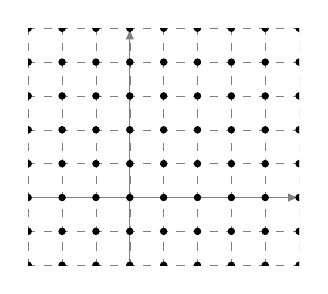
\begin{tikzpicture}[scale=0.43, every node/.style={scale=0.4}]
    \coordinate (Origin)   at (0,0);
    \coordinate (XAxisMin) at (-3,0);
    \coordinate (XAxisMax) at (5,0);
    \coordinate (YAxisMin) at (0,-2);
    \coordinate (YAxisMax) at (0,5);
    \draw [thin, gray,-latex] (XAxisMin) -- (XAxisMax);% Draw x axis
    \draw [thin, gray,-latex] (YAxisMin) -- (YAxisMax);% Draw y axis

    \clip (-3,-2) rectangle (5cm,5cm); % Clips the picture...
    \pgftransformscale{0.5}
          % This is actually the transformation matrix entries that
          % gives the slanted unit vectors. You might check it on
           % MATLAB etc. . I got it by guessing.
    \coordinate (Bone) at (0,2);
    \coordinate (Btwo) at (2,-2);
    \draw[style=help lines,dashed] (-10,-10) grid[step=2cm] (10,10);
          % Draws a grid in the new coordinates.
          %\filldraw[fill=gray, fill opacity=0.3, draw=black] (0,0) rectangle (2,2);
              % Puts the shaded rectangle
    \foreach \x in {-5,-4,...,5}{% Two indices running over each
      \foreach \y in {-5,-4,...,5}{% node on the grid we have drawn 
        \node[draw,circle,inner sep=2pt,fill] at (2*\x,2*\y) {};
            % Places a dot at those points
      }
    }
    %\draw [thin,-latex,red, fill=gray, fill opacity=0.3] (0,0)
        % -- ($2*(0,2)+(2,-2)$)
        % -- ($3*(0,2)+2*(2,-2)$) -- ($(0,2)+(2,-2)$) -- cycle;
  \end{tikzpicture}\ 
  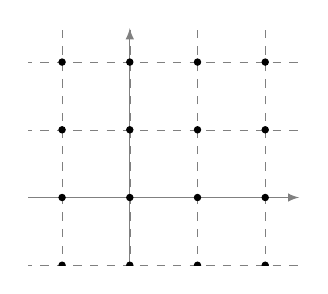
\begin{tikzpicture}[scale=0.43, every node/.style={scale=0.4}]
    \coordinate (Origin)   at (0,0);
    \coordinate (XAxisMin) at (-3,0);
    \coordinate (XAxisMax) at (5,0);
    \coordinate (YAxisMin) at (0,-2);
    \coordinate (YAxisMax) at (0,5);
    \draw [thin, gray,-latex] (XAxisMin) -- (XAxisMax);% Draw x axis
    \draw [thin, gray,-latex] (YAxisMin) -- (YAxisMax);% Draw y axis

    \clip (-3,-2) rectangle (5cm,5cm); % Clips the picture...
          % This is actually the transformation matrix entries that
          % gives the slanted unit vectors. You might check it on
           % MATLAB etc. . I got it by guessing.
    \coordinate (Bone) at (0,2);
    \coordinate (Btwo) at (2,-2);
    \draw[style=help lines,dashed] (-10,-10) grid[step=2cm] (10,10);
          % Draws a grid in the new coordinates.
          %\filldraw[fill=gray, fill opacity=0.3, draw=black] (0,0) rectangle (2,2);
              % Puts the shaded rectangle
    \foreach \x in {-5,-4,...,5}{% Two indices running over each
      \foreach \y in {-5,-4,...,5}{% node on the grid we have drawn 
        \node[draw,circle,inner sep=2pt,fill] at (2*\x,2*\y) {};
            % Places a dot at those points
      }
    }
    %\draw [thin,-latex,red, fill=gray, fill opacity=0.3] (0,0)
        % -- ($2*(0,2)+(2,-2)$)
        % -- ($3*(0,2)+2*(2,-2)$) -- ($(0,2)+(2,-2)$) -- cycle;
  \end{tikzpicture}\ 
  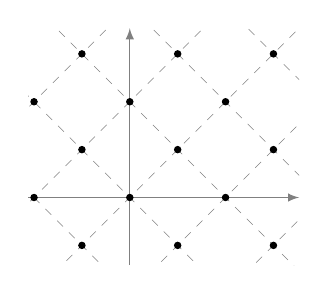
\begin{tikzpicture}[scale=0.43, every node/.style={scale=0.4}]
    \coordinate (Origin)   at (0,0);
    \coordinate (XAxisMin) at (-3,0);
    \coordinate (XAxisMax) at (5,0);
    \coordinate (YAxisMin) at (0,-2);
    \coordinate (YAxisMax) at (0,5);
    \draw [thin, gray,-latex] (XAxisMin) -- (XAxisMax);% Draw x axis
    \draw [thin, gray,-latex] (YAxisMin) -- (YAxisMax);% Draw y axis

    \clip (-3,-2) rectangle (5cm,5cm); % Clips the picture...
    \pgftransformrotate{45}
          % This is actually the transformation matrix entries that
          % gives the slanted unit vectors. You might check it on
           % MATLAB etc. . I got it by guessing.
    \coordinate (Bone) at (0,2);
    \coordinate (Btwo) at (2,-2);
    \draw[style=help lines,dashed] (-10,-10) grid[step=2cm] (10,10);
          % Draws a grid in the new coordinates.
          %\filldraw[fill=gray, fill opacity=0.3, draw=black] (0,0) rectangle (2,2);
              % Puts the shaded rectangle
    \foreach \x in {-5,-4,...,5}{% Two indices running over each
      \foreach \y in {-5,-4,...,5}{% node on the grid we have drawn 
        \node[draw,circle,inner sep=2pt,fill] at (2*\x,2*\y) {};
            % Places a dot at those points
      }
    }
    %\draw [thin,-latex,red, fill=gray, fill opacity=0.3] (0,0)
        % -- ($2*(0,2)+(2,-2)$)
        % -- ($3*(0,2)+2*(2,-2)$) -- ($(0,2)+(2,-2)$) -- cycle;
  \end{tikzpicture}
}
\visible<3->{Every lattice is homothetic to one of the form $\ZZ + \ZZ\tau$ for some $\tau \in \CC$ with positive imaginary part.}
\end{frame}

\begin{frame}{The $j$-invariant}
\note{
The hyper-alert among you might have recognised the number 744 from the first slides
}
The $j$-invariant is a function
\[
j\colon\{\text{lattices}\} \to \CC
\]
such that $j(L) = j(L') \iff L$ and $L'$ are homothetic.

\visible<2->{We can define $j$ on the upper half plane by $j(\tau) = j(\ZZ + \ZZ\tau)$.
Letting $q = e^{2\pi i \tau}$ we have
\begin{align*}
j(\tau) = q^{-1} &+ 744 + 196884q + 21493760q^2 \\
&+ 864299970q^3 + 20245856256q^4 + \cdots.\
\end{align*}}
\end{frame}

\begin{frame}{The $j$-invariant}
\begin{figure}
\includegraphics[width=\textwidth, trim=1600 0 1600 0, clip]{img/j.png}
\caption{\label{jinv}The $j$-invariant, picture by Fredrik Johansson}
\end{figure}
\end{frame}

\section{Singular moduli}
\begin{frame}{Singular moduli}
\begin{block}{Definition}
The values $j(\tau)$ for $\tau$ imaginary quadratic are called \emph{singular moduli}.
\end{block}
\visible<2->
{
\begin{block}{Examples}
\begin{align*}
j(i) &= 1728,\\
j\left(\frac{1 + \sqrt{-3}}{2}\right) &= 0,\\
j\left(\frac{1 + \sqrt{-15}}{2}\right) &= \frac{-191025 - 85995 \sqrt{5}}{2}.
\end{align*}
\end{block}
}
\end{frame}

\begin{frame}{(A corollary of) The first main theorem of class field theory}
\begin{block}{Theorem}
If $K$ is an imaginary quadratic field, $\ZZ_K = \ZZ + \ZZ\tau$ then:
\begin{enumerate}
\item $j(\tau)$ is an algebraic integer.
\pause\item The Hilbert class field of $K$ is $K(j(\tau))$.
\end{enumerate}
\end{block}
\pause
\begin{block}{A (partial) converse (Schneider)}
If $\tau$ is an algebraic number that is not imaginary quadratic then $j(\tau)$ is transcendental.
\end{block}
\end{frame}

\begin{frame}{Explaining Hermite's observations}
\begin{gather*}
K = \QQ(\sqrt{-d}) \text{ with } \cl(\ZZ_K) = 1,\ \ZZ_K = \ZZ+\ZZ\tau.\\
\visible<2->{\Downarrow}\\
\visible<2->{\text{The Hilbert class field of $K$ is $K$}.}\\
\visible<3->{\Downarrow}\\
\visible<3->{j(\tau)\in \ZZ_K.}\\
\visible<4->{\Downarrow}\\
\visible<4->{e^{-2\pi i \tau} + 744 + 196884 e^{2\pi i \tau} + \ldots\in \ZZ_K\cap \RR}\visible<5->{ = \ZZ.}
\end{gather*}
\end{frame}

\begin{frame}{Explaining Hermite's observations}
So if $d= 163$ we have $\tau = (1 + \sqrt{-163})/2$
\visible<2->{and so
\begin{align*}
j(\tau) &= e^{-\pi i (1 + i\sqrt{163})} + 744 + 196884 e^{\pi i (1+i\sqrt{163})} + \ldots\\
&= -e^{\pi\sqrt{163}} + 744 - 196884 e^{-\pi\sqrt{163}} + \ldots
\end{align*}
is an integer.
}

\visible<3->{The trailing terms are tiny here giving
\[
e^{\pi\sqrt{163}} \approx -j(\tau) + 744.
\]
}
\end{frame}

\begin{frame}{The class number 1 problem}
\begin{block}{Theorem (Stark-Heegner)}
The only imaginary quadratic number fields with trivial class group are $\QQ(\sqrt{-d})$ for
\[d\in\{1,2,3,7,11,19,43,67,163\}.\]
\end{block}
\pause
So we expect $e^{\pi\sqrt{19}}$ to be close to an integer too:
\[
e^{\pi\sqrt{19}} = .
\]
\pause The value is not as close as $e^{-\pi\sqrt{d}}$ has larger absolute value for smaller $d$.
\end{frame}

\section{Modern work}
\begin{frame}{A formula of Gross-Zagier}
We have that $j() = $ and $j() = $ and so
\[
j(\sqrt{}) - j(\sqrt{}) = .
\]


\end{frame}

\begin{frame}{A formula of Gross-Zagier}
\begin{block}{Theorem (Gross-Zagier, '84)}
\end{block}
\end{frame}

\section{Conclusion}
\begin{frame}{Closing remarks}
\note{just specific values of a well studied function}
\begin{itemize}
\item Singular moduli are not particularly complex objects in and of themselves.
\pause \item But their relation between different areas of mathematics ensures that they are still a research topic to this day.
\end{itemize}
\end{frame}

\begin{frame}{Sources}
I used some of the following when preparing this talk, and so they are probably good places to look to learn more about the topic:
\begin{itemize}
\item ``Primes of the form $x^2 + ny^2$'' -- David A. Cox
\end{itemize}
\end{frame}

\end{document}


